\subsection{Purpose}

Task D evaluates the harmonic lattice dynamics of the relaxed magnetic
ground-state structures identified in Task B.  For Ni, the phonon calculation
uses the relaxed ferromagnetic PBE structure.  For NiO, the calculation uses
the relaxed DFT+\(U\) AFM-II structure, because this is the lowest-energy NiO
state considered in Task B.

\subsection{Computational Setup}

The phonon calculations use the finite-difference force-constant workflow in
VASP.  In this approach, VASP displaces atoms in a supercell, computes the
resulting forces, constructs the second-order force constants, and diagonalizes
the dynamical matrix.  The finite-difference setup uses \texttt{IBRION = 6},
\texttt{NFREE = 2}, and \texttt{POTIM = 0.015}~\AA.  The use of
\texttt{IBRION = 6} lets VASP reduce the number of displacements by symmetry
where possible \cite{vasp-phonon-fd}.

Both systems use \(2\times2\times2\) phonon supercells constructed from the
relaxed Task B cells.  The Ni supercell contains 32 Ni atoms and uses a
\(12\times12\times12\) electronic k-point mesh.  The NiO supercell contains 16
Ni atoms and 16 O atoms and uses an \(8\times8\times8\) electronic k-point mesh.
These k-point meshes preserve approximately the same reciprocal-space sampling
density as the smaller cells used in Tasks B and C.  The phonon dispersion and
phonon density of states are obtained by reading the calculated force constants
from \texttt{vaspout.h5}, supplying a \texttt{QPOINTS} path or mesh, and setting
\texttt{LPHON\_DISPERSION} or \texttt{PHON\_DOS}, respectively
\cite{vasp-phonon-dispersion}.

For NiO, a separate primitive-cell linear-response calculation with
\texttt{LEPSILON = .TRUE.} is included to compute the ion-clamped dielectric
tensor and Born effective charge tensors.  These quantities are passed to the
phonon runs through \texttt{LPHON\_POLAR}, \texttt{PHON\_DIELECTRIC}, and
\texttt{PHON\_BORN\_CHARGES} so that the long-range dipole contribution and
LO-TO splitting can be treated in the polar oxide \cite{vasp-phonon-dispersion,
vasp-lepsilon}.

\subsection{Prepared Workflow}

The Task D input folders are:
\begin{itemize}
  \item \texttt{Ni/D/PBE\_FM}: ferromagnetic Ni phonons;
  \item \texttt{NiO/D/DFTU\_AFM}: AFM-II DFT+\(U\) NiO phonons.
\end{itemize}
Each case contains \texttt{force\_constants}, \texttt{dispersion}, and
\texttt{dos} subfolders.  The NiO case also contains a \texttt{dielectric}
subfolder used to generate the polar correction input.

After the VASP jobs finish, the analysis script
\texttt{common/D/analyze\_task\_d.py} extracts the \(\Gamma\)-point
frequencies, identifies imaginary modes, writes the summary tables, and creates
the phonon dispersion and PhDOS plots.

\subsection{Results}

The Task D VASP calculations have to be run before numerical phonon results can
be inserted.  The expected output tables are written to
\texttt{outputs/D/reports/Task\_D\_summary\_table.md} and
\texttt{outputs/D/reports/Task\_D\_gamma\_modes.md}.

\IfFileExists{figures/Ni_PBE_FM_phonon_dispersion.pdf}{%
\begin{figure}[htbp]
\centering
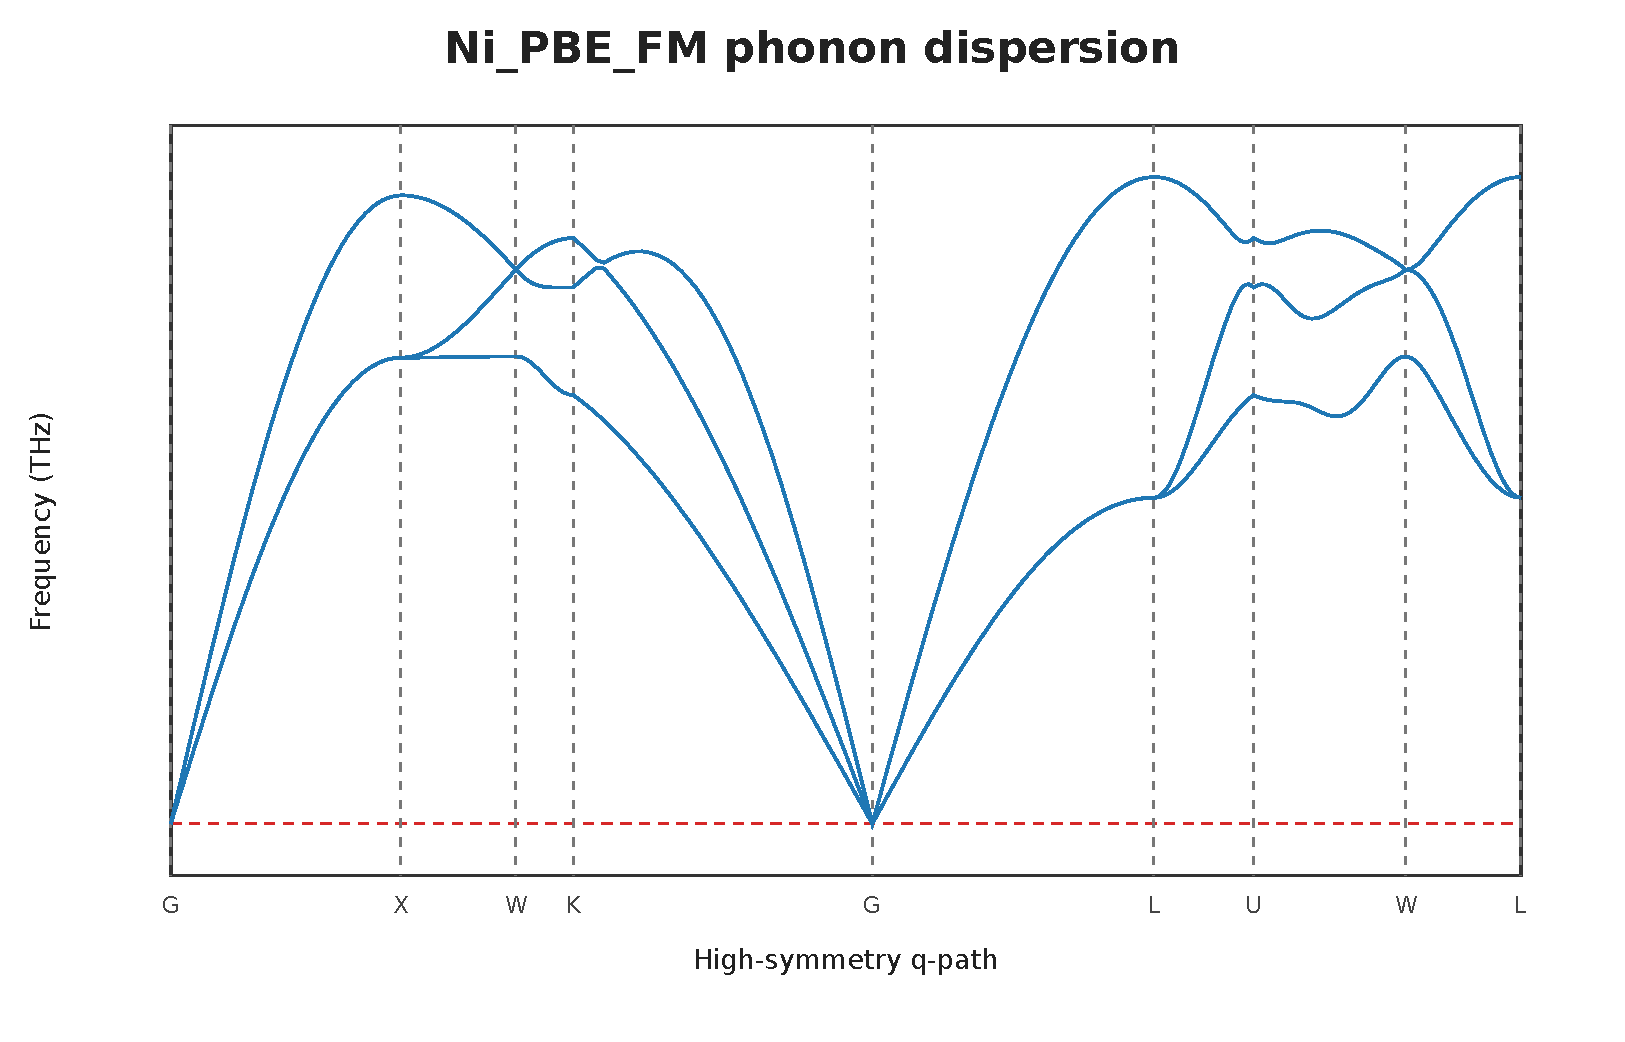
\includegraphics[width=\textwidth]{figures/Ni_PBE_FM_phonon_dispersion.pdf}
\caption{Phonon dispersion for relaxed ferromagnetic PBE Ni.}
\label{fig:task-d-ni-dispersion}
\end{figure}
}{}

\IfFileExists{figures/Ni_PBE_FM_phdos.pdf}{%
\begin{figure}[htbp]
\centering
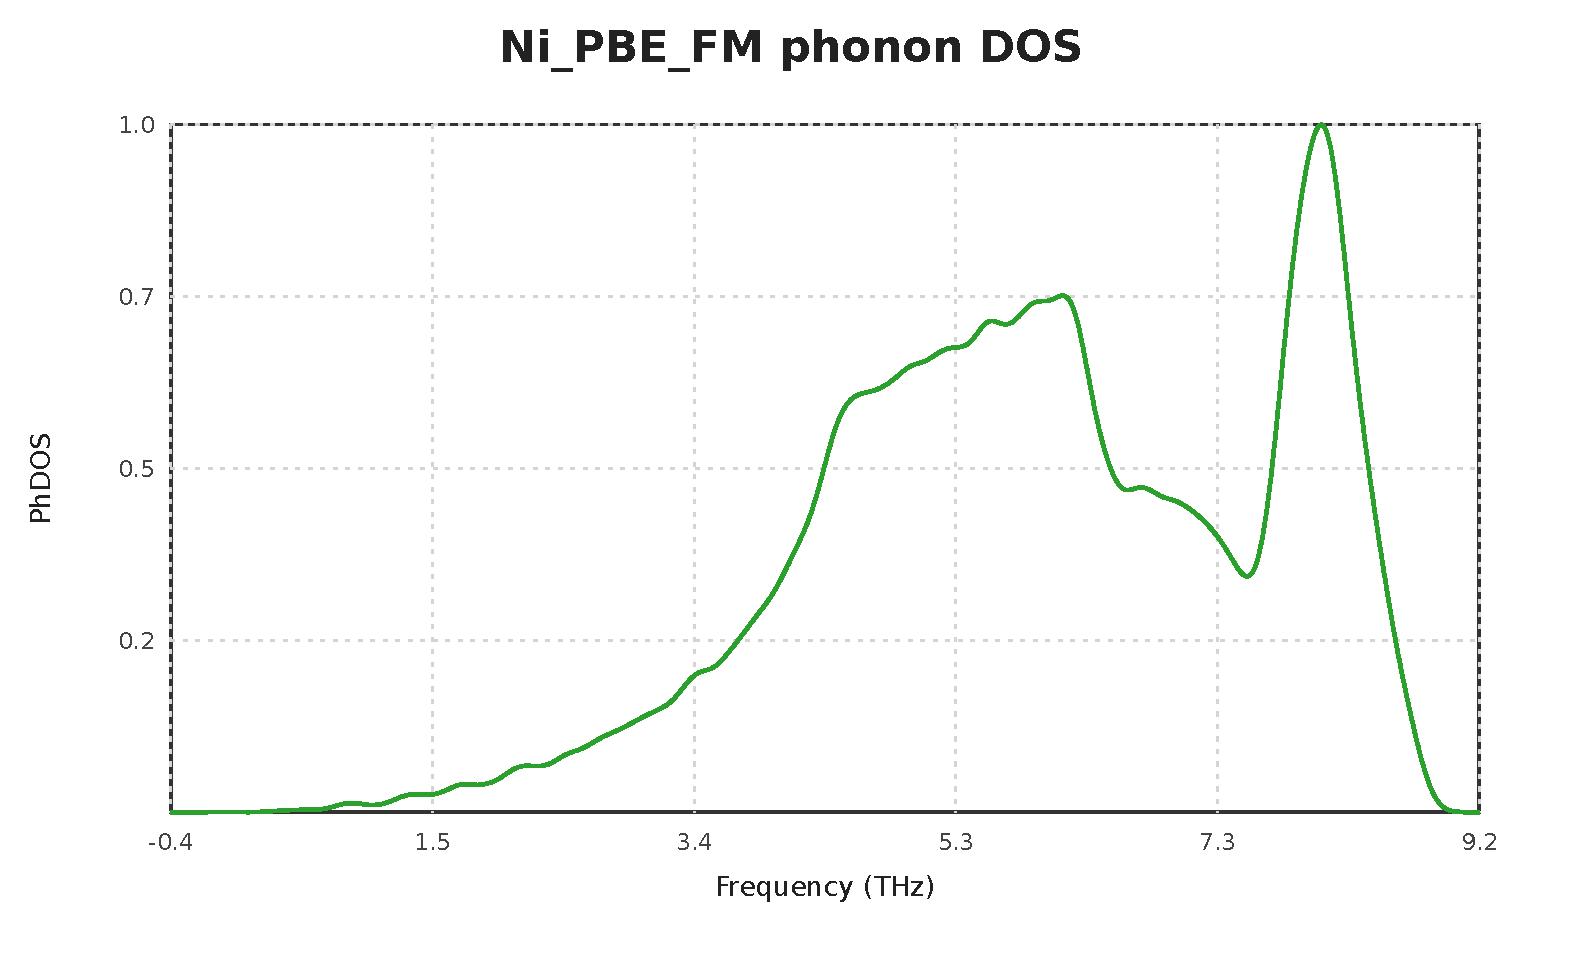
\includegraphics[width=\textwidth]{figures/Ni_PBE_FM_phdos.pdf}
\caption{Phonon density of states for relaxed ferromagnetic PBE Ni.}
\label{fig:task-d-ni-phdos}
\end{figure}
}{}

\IfFileExists{figures/NiO_DFTU_AFM_phonon_dispersion.pdf}{%
\begin{figure}[htbp]
\centering
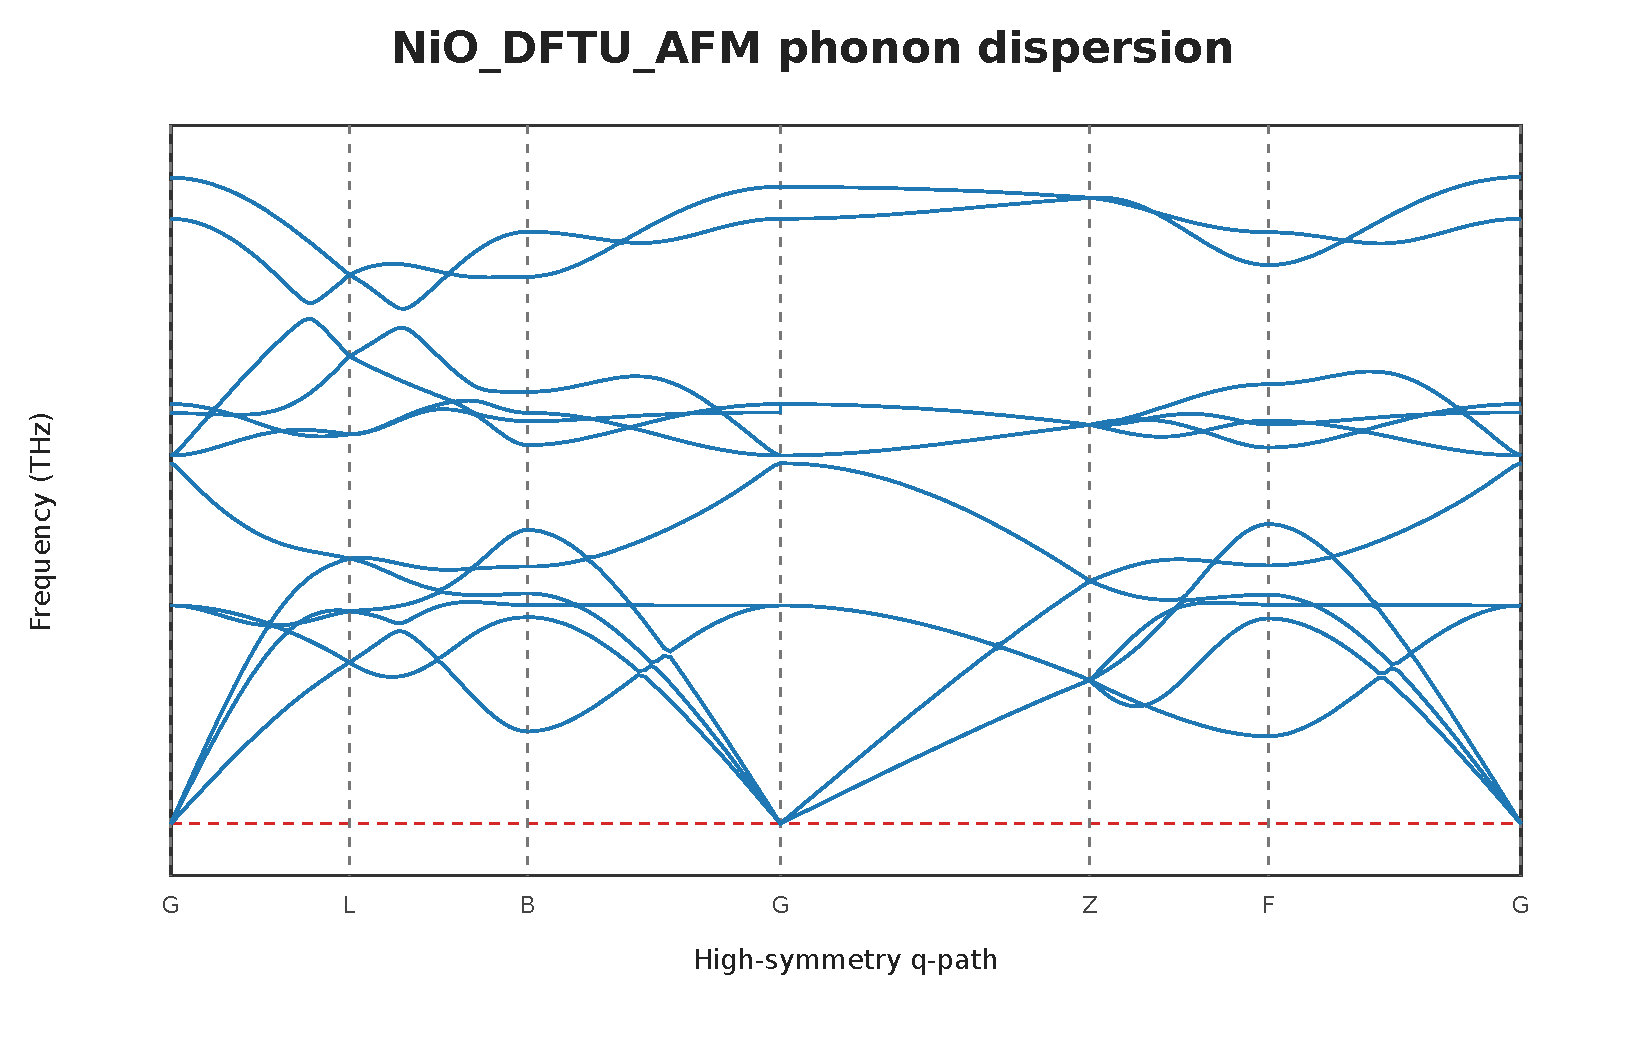
\includegraphics[width=\textwidth]{figures/NiO_DFTU_AFM_phonon_dispersion.pdf}
\caption{Phonon dispersion for relaxed DFT+\(U\) NiO in the AFM-II magnetic
ordering.}
\label{fig:task-d-nio-dispersion}
\end{figure}
}{}

\IfFileExists{figures/NiO_DFTU_AFM_phdos.pdf}{%
\begin{figure}[htbp]
\centering
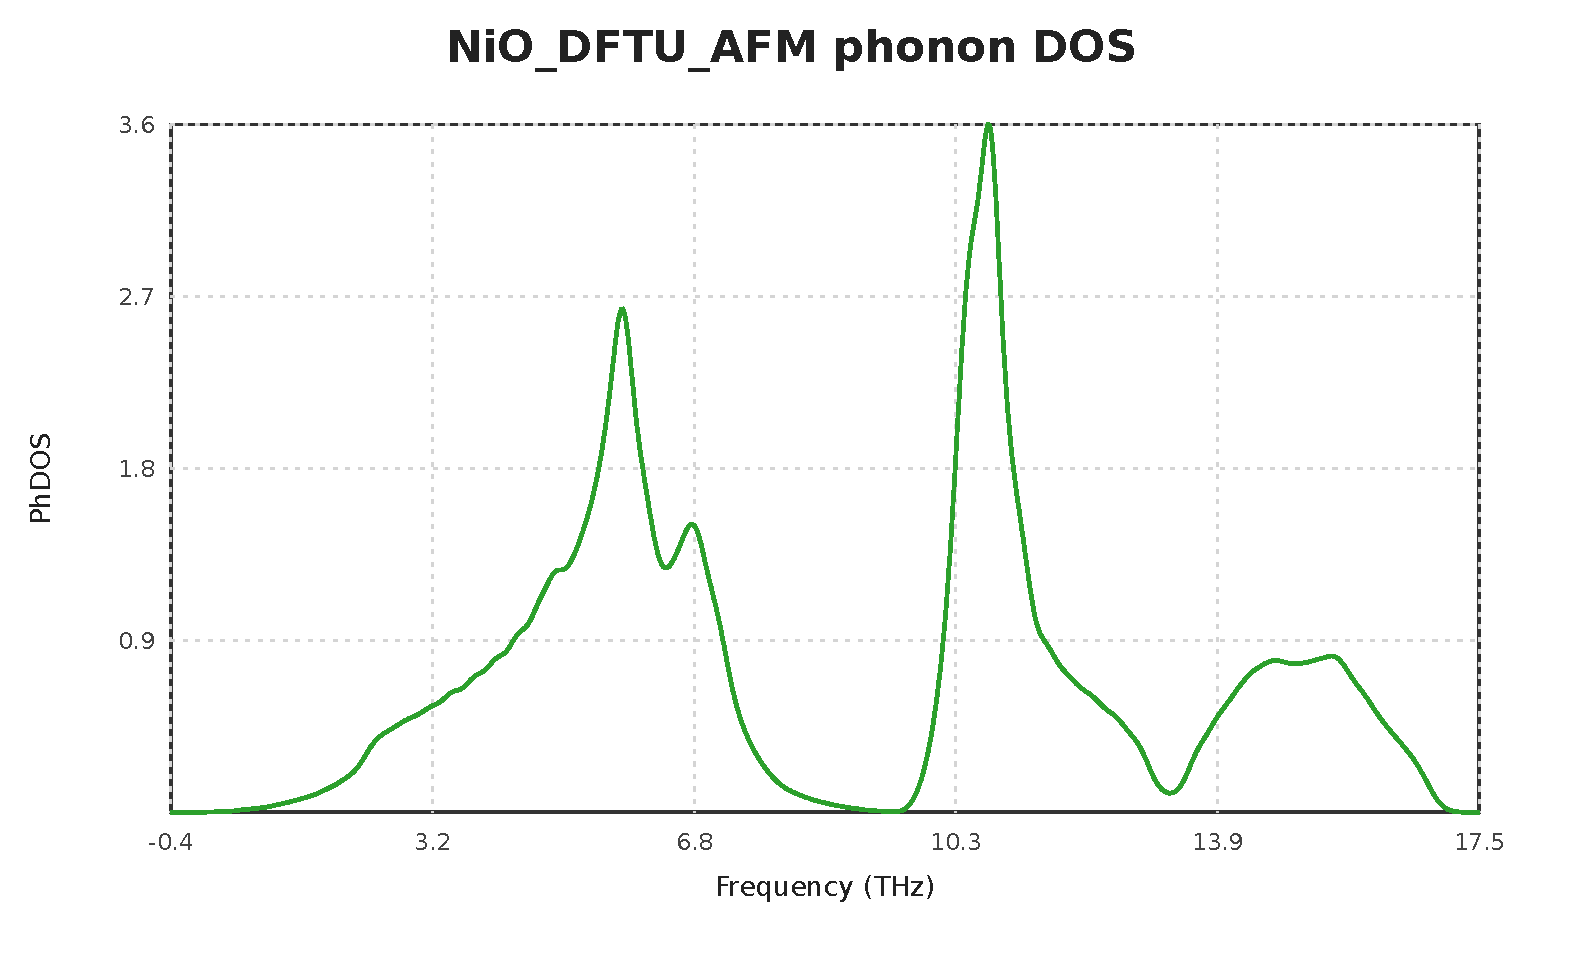
\includegraphics[width=\textwidth]{figures/NiO_DFTU_AFM_phdos.pdf}
\caption{Phonon density of states for relaxed DFT+\(U\) NiO in the AFM-II
magnetic ordering.}
\label{fig:task-d-nio-phdos}
\end{figure}
}{}

\subsection{Discussion}

The phonon spectra should be interpreted by checking whether any branch has a
negative frequency, equivalently an imaginary mode.  If no significant
imaginary frequencies are present, the relaxed structure is dynamically stable
within the harmonic approximation.  Small residual imaginary acoustic
frequencies near \(\Gamma\) can occur from finite numerical precision, limited
supercell size, or incomplete force convergence; if they appear, the first
checks should be a larger supercell, tighter electronic convergence, and denser
k-point sampling \cite{vasp-phonon-fd}.
